\chapter{システム}
本章では,日常生活動作別の時間記録アプリケーション,ADLoggerを提案する.
はじめにADLoggerシステムの概要を述べ,次にADLoggerの特徴を説明する.
そして最後に,ユーザがADLoggerを利用する流れについて述べる.

\section{ADLoggerシステムの概要}
ADLoggerはユーザの行動名別に経過時間を記録するiOSアプリケーションである.
ユーザは行動名毎に行動時間を実測で記録される.
予測算出画面では,行動別の平均時間がリスト形式でカラム毎に出力される.
カラムを複数選択する事で複数行動を行う際の必要時間を計算・可視化する事が可能である.

\section{ADLoggerシステムの特徴}
本節では,ADLoggerシステムの特徴としてあげられる機能を挙げる.

\subsection{タスク別ストップウォッチ記録}
内蔵されているストップウォッチで行動名毎に行動時間を実測で記録される.
実測値を記録する為,個人の見積もり精度に依らない数値を取得することが可能である.

\subsection{各時間予測}
各行動を下記の計算方法を用いてユーザの行動別記録時間の標準的な時間を算出し,リスト形式で行動別に表示する.
リストのカラムをタップすると,選択された行動の合計の必要時間を下記の計算手法を元に算出する.
これにより簡単に複数タスクに対する必要時間見込みを簡単に把握する事が可能となる.
算出された合計時間はAppleのカレンダーに登録が可能であり,Appleカレンダーに登録された既存の予定と同時に閲覧することが可能である.


\section{平均時間の算出方法}
システム上の各タスク毎の見積もり及びバッファの定め方に関して記述する.
\subsection{各時間予測}
タスク完了に要する時間の期待時間を$\bar{T}$,記録時間を$T$とすると,数式(\ref{T})の様に平均時間を用いて各タスクの見積もりを行う.
また標準偏差の信頼範囲に則り,各タスクの標準偏差$\sigma (T)$に$N (N=0〜3)$を掛けたものを変動バッファ$Tv$と定義した(数式(\ref{Tv})).
\begin{equation}
\label{T}
\bar{T}=\frac{1}{n}\displaystyle\sum_{i=1}^{n}T_{i}
\end{equation}

\begin{eqnarray}
\label{Tv}
Tv=\sigma (T)×N \\
(N= 0, 1,2, 3 )\nonumber
\end{eqnarray}

\subsection{合計時間の算出}

合計時間の予測を出すにはまず先ほど算出したタスク毎の$\bar{T}$と$Tv$し,更にユーザが自分で決定し数値として入力ができる固定バッファ$Tf$を足す事で算出する(数式(\ref{Ts})).
\begin{equation}
\label{Ts}
T_{sum}= \displaystyle\sum_{i=1}^{n} (\bar{T}_{i} + Tv_{i})+Tf
\end{equation}


\section{ADLoggerシステムの使用方法}
本アプリケーションを開くと,トップ画面が開かれる(図~\ref{fig:top}).
``LOGIN"ボタンを押すとユーザ名とパスワードが求められる(図~\ref{fig:login}).
初回の場合は下段の``REGISTERATION"ボタンから登録画面に移行し登録を行う(図~\ref{fig:reg}).
ログインが成功するとメイン画面に移行する(図~\ref{fig:ltop}).
尚,初回以降は直接メイン画面に移行する事が可能である.

メイン画面の``TIMER"ボタンにからは,行動を記録する事が可能である.
``TIMER"ボタンを押すと,``START"ボタンのあるストップウォッチ画面が現れる(図~\ref{fig:stopwatch}).
``START"ボタンを押すと``START"ボタンが``STOP"ボタンに切り替わった後,ストップウォッチが起動し時間を計測できる.
計測後は``STOP"ボタンを押す.出力されるアラートの中から``終了"ボタンを選択し,タスク名選択画面に移行する(図~\ref{fig:list}).
尚,記録を破棄したい場合はアラートの``Reset"ボタンを,ストップウォッチを止めたくない場合は``計測に戻る"を選択する.

タスク選択画面では行動名がリスト形式で表示されている.一度でも登録された行動名であれば行動名を選択する事で経過時間を保存する事ができる.
新たな行動名であれば``新規追加"ボタンを押し,出力されたアラートに行動名を入力し名前を登録後上記同様に保存する.

一度でも記録時間が保存されると``ADLog"ボタンから行動記録を閲覧する事が可能である(図~\ref{fig:log}).
ユーザは必要に応じてタスクを選択しする事で,複数タスクの合計時間を変動バッファ(中央下色がついている数値)・固定バッファ(中央下黒色の数値)を適宜調整しながら見る事が可能である.

右上のカレンダーのアイコンをクリックすると,カレンダー登録画面(図~\ref{fig:calendar})に遷移する.
画面上のタスク名,日付,登録時間に対する開始時刻/終了時刻を入力し``追加"ボタンを押すとAppleのカレンダーに記入した時刻が登録できる.

利用規約,実験の説明%アプリも
,アンケート,設定に関してはトップ画面(図~\ref{fig:top})の``HELP"ボタン先の画面で管理する(図~\ref{fig:help}).
アンケート画面は各タスクかかった時間と全てのタスクを連続でやった時の総時間の予測を記入してもらうものである(図~\ref{fig:survey1},図~\ref{fig:survey2}).
設定画面は変動バッファと固定バッファの調整を行うことが出来る図~\ref{fig:setting}.
また,後述する実験の関係上,ADLoggerボタンから行動記録の閲覧とストップウォッチスタート時のカウントアップの閲覧に関しても設定画面から制御できるようにした.

\begin{figure}[ht]
\begin{center}
\begin{tabular}{c}

	\begin{minipage}[b]{0.5\linewidth}
	\begin{center}
		\fbox{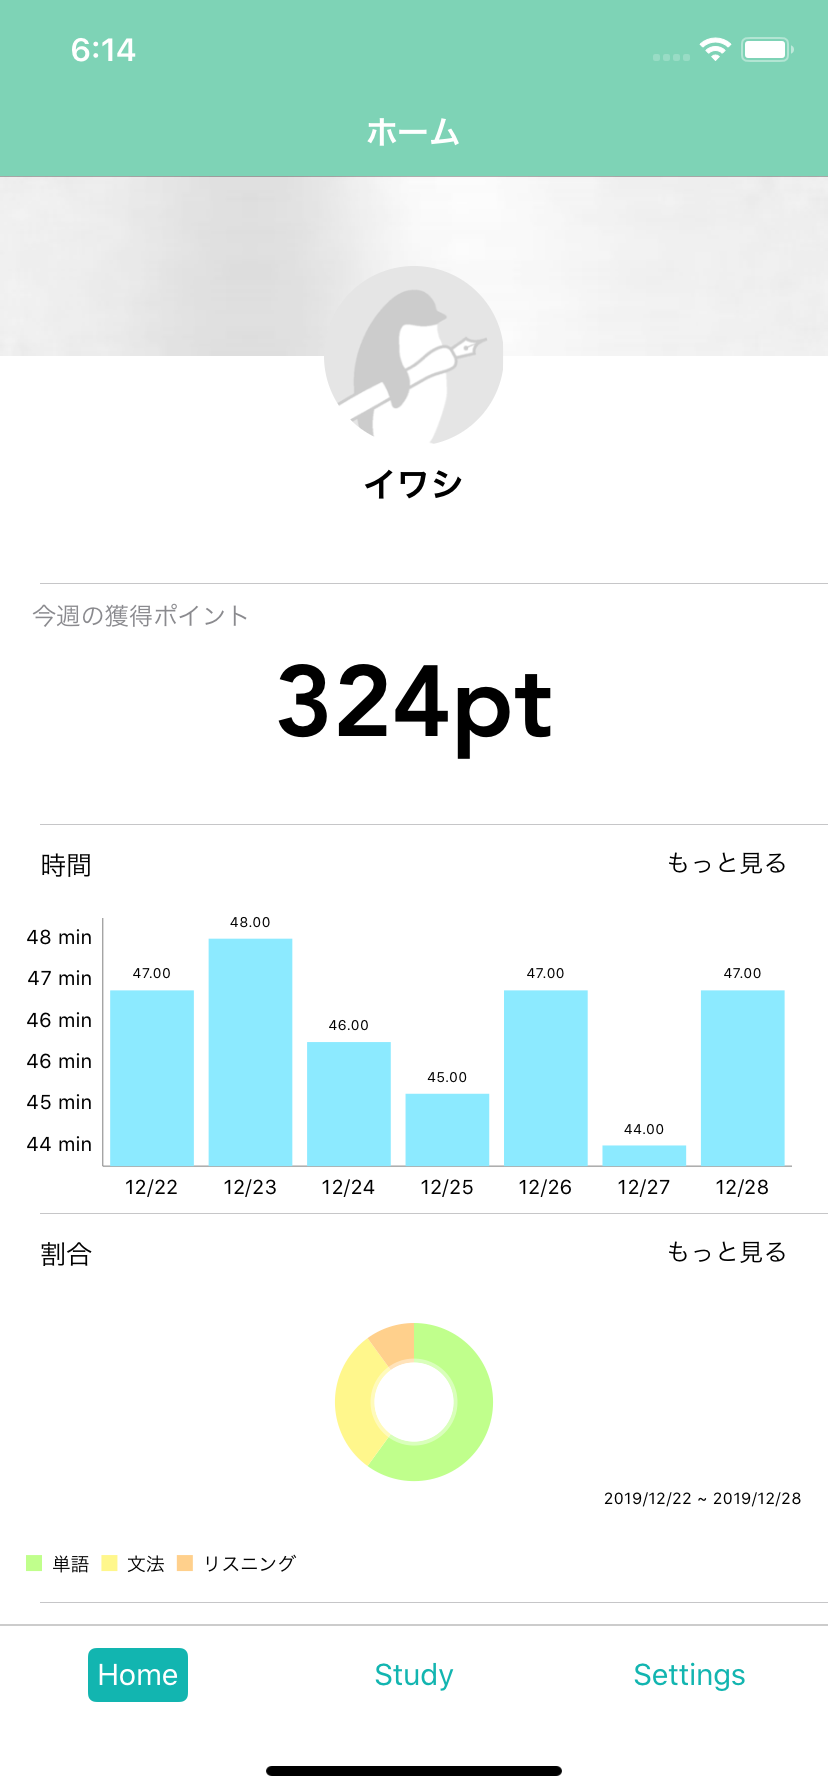
\includegraphics[width=5cm]{images/4/top.png}}
		\caption{トップ画面}
		\label{fig:top}
	\end{center}
  	\end{minipage}

	\begin{minipage}[b]{0.5\linewidth}
	\begin{center}
		\fbox{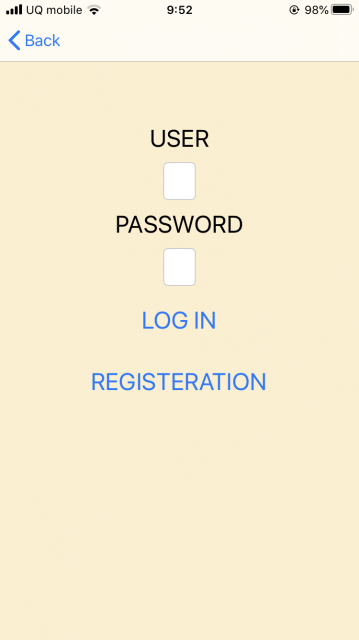
\includegraphics[width=5cm]{images/4/login.png}}
		\caption{ログイン画面}
		\label{fig:login}
	\end{center}
  	\end{minipage}
	
	\\
	
	\begin{minipage}[b]{0.5\linewidth}
	\begin{center}
		\fbox{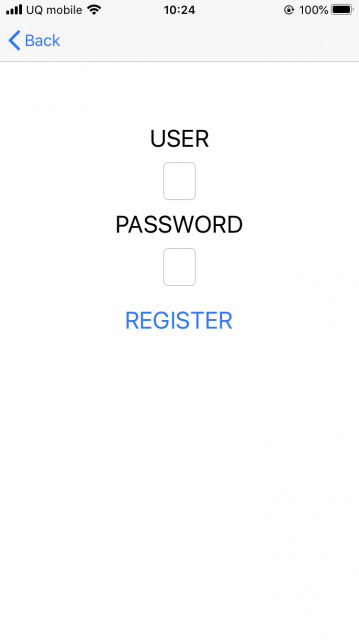
\includegraphics[width=5cm]{images/4/reg.png}}
		\caption{登録画面}
		\label{fig:reg}
	\end{center}
  	\end{minipage}
	
	\begin{minipage}[b]{0.5\linewidth}
	\begin{center}
		\fbox{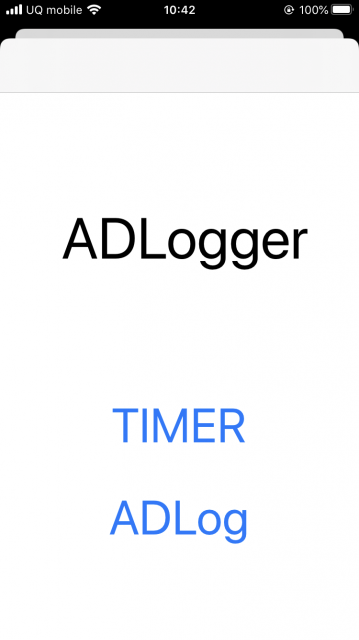
\includegraphics[width=5cm]{images/4/ltop.png}}
		\caption{メイン画面}
		\label{fig:ltop}
	\end{center}
  	\end{minipage}
	
  	\end{tabular}
  \end{center}
\end{figure}


\begin{figure}[ht]
\begin{center}
\begin{tabular}{c}

	\begin{minipage}[b]{0.5\linewidth}
	\begin{center}
		\fbox{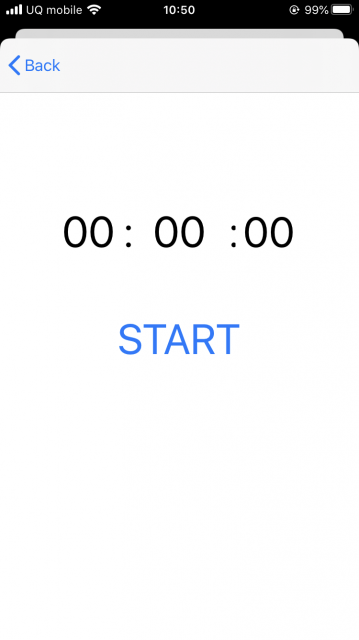
\includegraphics[width=5cm]{images/4/stopwatch.png}}
		\caption{ストップウォッチ画面}
		\label{fig:stopwatch}
	\end{center}
  	\end{minipage}
	
	\begin{minipage}[b]{0.5\linewidth}
	\begin{center}
		\fbox{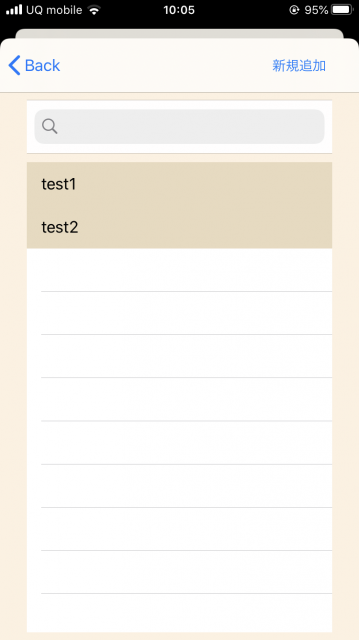
\includegraphics[width=5cm]{images/4/list.png}}
		\caption{タスク選択画面}
		\label{fig:list}
	\end{center}
  	\end{minipage}
	
	\\
	\begin{minipage}[b]{0.5\linewidth}
	\begin{center}
		\fbox{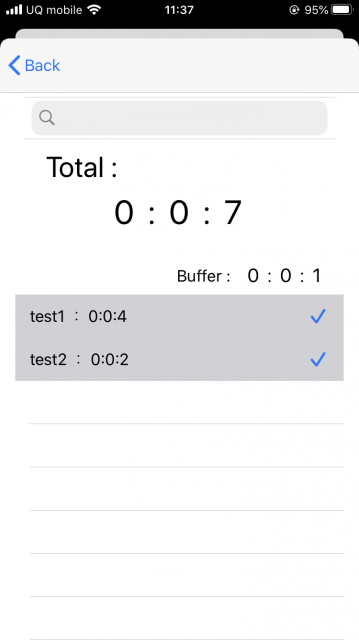
\includegraphics[width=5cm]{images/4/log.png}}
		\caption{ADLog計算出力画面例}
		\label{fig:log}
	\end{center}
  	\end{minipage}
	
	\begin{minipage}[b]{0.5\linewidth}
	\begin{center}
		\fbox{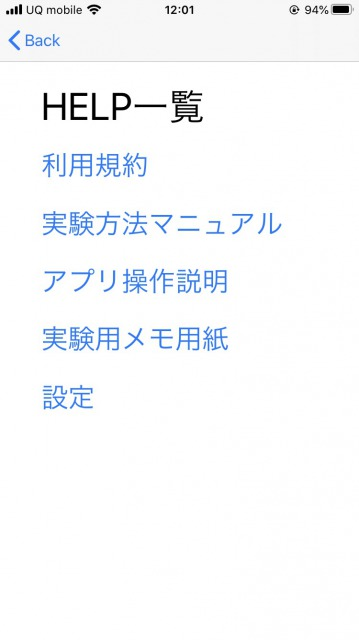
\includegraphics[width=5cm]{images/4/help.png}}
		\caption{HELP画面}
		\label{fig:help}
	\end{center}
  	\end{minipage}
	
  	\end{tabular}
  \end{center}
\end{figure}

\begin{figure}[ht]
\begin{center}
\begin{tabular}{c}

	\begin{minipage}[b]{0.5\linewidth}
	\begin{center}
		\fbox{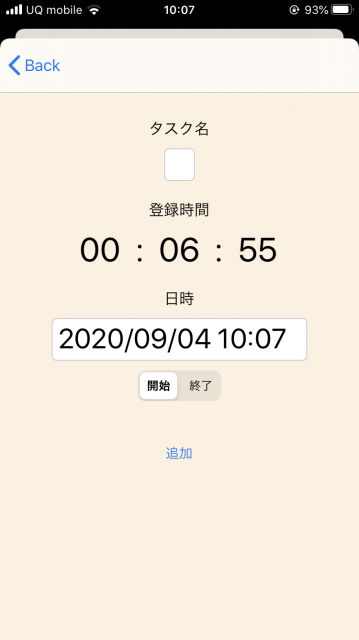
\includegraphics[width=5cm]{images/4/calendar.png}}
		\caption{カレンダー登録画面}
		\label{fig:calendar}
	\end{center}
  	\end{minipage}

	\begin{minipage}[b]{0.5\linewidth}
	\begin{center}
		\fbox{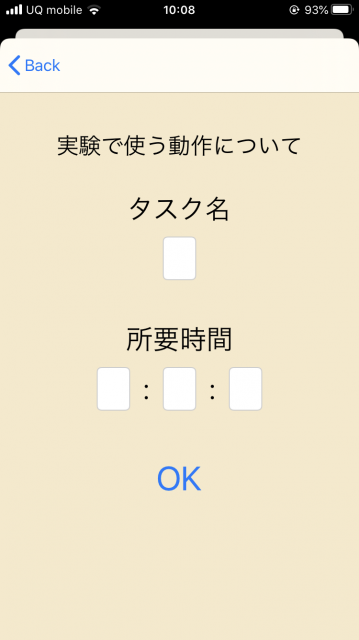
\includegraphics[width=5cm]{images/4/survey1.png}}
		\caption{アンケート画面1}
		\label{fig:survey1}
	\end{center}
  	\end{minipage}
	
	\\
	\begin{minipage}[b]{0.5\linewidth}
	\begin{center}
		\fbox{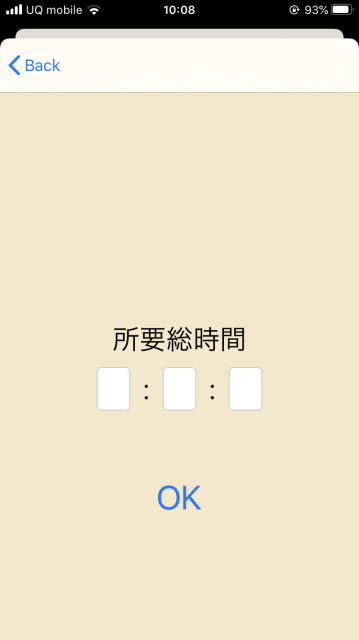
\includegraphics[width=5cm]{images/4/survey2.png}}
		\caption{アンケート画面2}
		\label{fig:survey2}
	\end{center}
  	\end{minipage}
	
		\begin{minipage}[b]{0.5\linewidth}
	\begin{center}
		\fbox{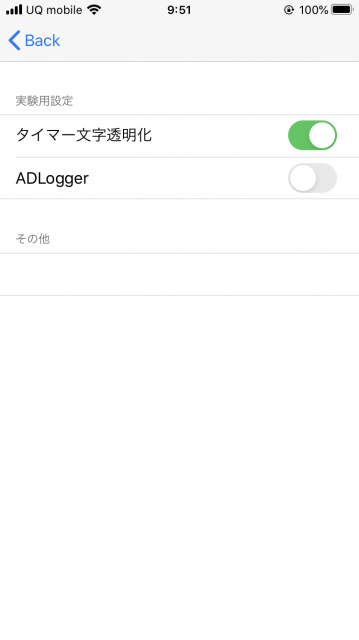
\includegraphics[width=5cm]{images/4/setting.png}}
		\caption{設定画面}
		\label{fig:setting}
	\end{center}
  	\end{minipage}
	
  	\end{tabular}
  \end{center}
\end{figure}


\section{まとめ}
本章では,日常生活動作別行動時間記録及びリマインドを目的としたADLoggerシステムを提案した.
また,ADLoggerシステムの特徴および使用方法を述べた.
次章では,本システムの設計について述べる.